%% Neurocomputing (Elsevier) -- elsarticle template
%% Empirical study / negative result
%% Revised 2026-11-22: author list, verified bibliography, statistics recomputed
%% from per-seed evaluation records (see recompute_stats.py).

\documentclass[preprint,12pt]{elsarticle}

\usepackage{amsmath,amssymb}
\usepackage{amsthm}
\newtheorem{proposition}{Proposition}
\usepackage{graphicx}
\usepackage{booktabs}
\usepackage{algorithm}
\usepackage{algpseudocode}
\usepackage{hyperref}
\usepackage{xcolor}

\algrenewcommand\algorithmicrequire{\textbf{Input:}}
\algrenewcommand\algorithmicensure{\textbf{Output:}}

% natbib is loaded by elsarticle v3.5 itself; configure it here
\biboptions{numbers,sort&compress}

\journal{Neurocomputing}

% reference list set one size below the 12pt body (journal convention)
\renewcommand{\bibfont}{\footnotesize}

\begin{document}

\begin{frontmatter}

\title{Error-Aware Rank Allocation Collapses to Norm-Aware Allocation in 4--8-Bit LoRA:\\
A Cross-Quantizer Empirical Audit}

\author[inst1]{Yibo Zhang\corref{cor1}}
\ead{zhang_yibo@ahsgs.uum.edu.my}
\author[inst1]{Muhammad Syafiq bin Mohd Pozi}
\author[inst1]{Osman B Ghazali}
\cortext[cor1]{Corresponding author.}
\address[inst1]{School of Computing, Universiti Utara Malaysia,\\
06010 UUM Sintok, Kedah Darul Aman, Malaysia}

\begin{abstract}
Error-aware rank allocation assigns LoRA ranks in proportion to the product of per-layer quantization error and parameter importance, assuming that layers losing more information to compression benefit from larger ranks. We audit this assumption on Llama-3-8B across NF4, INT4-RTN and INT8 quantization with three to twelve training seeds per configuration. First, the allocation score is algebraically identical to the Frobenius norm of the quantization error matrix; because per-layer relative error is nearly constant at 4 bits (coefficient of variation 1.48\% for NF4, 0.48\% for INT4-RTN), the score correlates with the weight norm at $\rho = 0.998$ and the realised allocation is norm-proportional. Second, seed-matched paired analysis with Benjamini--Hochberg control shows no significant difference between error-aware and uniform allocation on MMLU or GSM8K ($q \geq 0.20$); equivalence testing bounds the MMLU difference within $\pm 0.5$ percentage points for all three quantizers, and the GSM8K difference within $\pm 2$ points for both 4-bit schemes. Relative error becomes forty times more dispersed under INT8 without regaining discriminative power, because it stays uncorrelated with weight norm ($|\rho| < 0.09$). Within the effect range our design resolves, error-aware rank allocation offers no measurable gain over uniform allocation; we state the sample sizes needed to settle smaller effects.
\end{abstract}

\begin{keyword}
quantized fine-tuning \sep LoRA \sep rank allocation \sep negative result \sep equivalence testing
\end{keyword}

\end{frontmatter}

%% =============================================================================
\section{Introduction}
\label{sec:intro}

Parameter-efficient fine-tuning (PEFT) is the standard route for adapting large language models under tight memory budgets: adapters~\citep{houlsby2019adapters}, prefix and prompt tuning~\citep{li2021prefix,lester2021prompt}, their unification~\citep{he2022unified}, and low-rank adaptation (LoRA)~\citep{hu2022lora}, which dominates because its update merges into the frozen weights at inference.

LoRA fixes one rank for every adapted module, which invites the question of whether layers should receive different budgets. AdaLoRA~\citep{zhang2023adalora} allocates rank from singular-value sensitivity, DoRA~\citep{liu2024dora} separates magnitude from direction, and several variants redistribute or rescale rank across layers~\citep{meng2024pissa,kalajdzievski2023rslora,kopiczko2024vera,ploner2026variablerank}. In the quantized setting, where frozen weights are stored in four or eight bits~\citep{dettmers2023qlora,dettmers2022llmint8}, compression supplies a second signal: per-layer quantization error. Error-aware methods rank layers by the product of that error and an importance proxy~\citep{kim2024ralora,lee2025rilq}, on the intuition that layers losing more information should receive more capacity.

We ask a diagnostic question instead of proposing another rule: \emph{does error-aware allocation differ measurably from uniform allocation under realistic 4--8-bit quantization?} The answer is negative, and the reason is structural. The score equals the Frobenius norm of the error matrix by algebra (Proposition~\ref{prop:degeneracy}), and at 4 bits that quantity is almost a pure function of the weight norm, so error-aware allocation is norm-aware allocation in disguise. We contribute:
\begin{enumerate}
    \item a cross-quantizer measurement of per-layer relative error on Llama-3-8B, showing near-constant 4-bit profiles (CV 1.48\% and 0.48\%) and a far more dispersed INT8 profile (CV 61.1\%) that stays uncorrelated with weight norm;
    \item the identity $s_l \equiv \|E_l\|_F$, making the rule a monotone transform of the error norm and, under the measured constancy of $\varepsilon_l$, a norm-proportional rule;
    \item a seed-matched audit over three quantizers and two benchmarks ($n = 3$--$12$) with false-discovery-rate control: no cell is significant ($q \geq 0.20$) and MMLU differences are equivalent within $\pm 0.5$ points;
    \item a cell-by-cell account of what the design resolves (minimum detectable effects 0.11--6.12 points) and the seeds needed to test a one-point effect (up to 26).
\end{enumerate}

The practical form of this result is a one-line diagnostic---the rank correlation between a candidate allocation statistic and the weight norm---which any method in this family can report before training.

%% =============================================================================
\section{Related Work}
\label{sec:related}

\textbf{Rank allocation.} AdaLoRA~\citep{zhang2023adalora} prunes singular values and redistributes budget, DoRA~\citep{liu2024dora} adapts magnitude and direction separately, PiSSA~\citep{meng2024pissa} initialises from principal components, LoRA+~\citep{hayou2024loraplus} uses asymmetric learning rates, VeRA~\citep{kopiczko2024vera} shares frozen projections, and rank-stabilised scaling removes sensitivity to the rank hyper-parameter~\citep{kalajdzievski2023rslora}. All of these presuppose that layers differ in how much rank they need, and we test one explicit instantiation of that presupposition.

\textbf{Quantized fine-tuning.} Post-training quantization compresses frozen weights~\citep{nagel2021whitepaper,gholami2021survey}; representative schemes are LLM.int8() \citep{dettmers2022llmint8}, GPTQ \citep{frantar2023gptq}, AWQ \citep{lin2024awq}, SmoothQuant \citep{xiao2023smoothquant}, ZeroQuant \citep{yao2022zeroquant} and QuIP \citep{chee2023quip}. QLoRA~\citep{dettmers2023qlora} pairs 4-bit NormalFloat storage with LoRA training and is the setting in which error-aware allocation has been proposed; LoftQ \citep{li2024loftq} instead reduces the mismatch between quantisation and low-rank training by alternating optimisation. Our audit fixes the storage scheme and varies only the allocation rule.

\textbf{Error-aware adaptation.} RA-LoRA~\citep{kim2024ralora} allocates rank for 2-bit models, RILQ~\citep{lee2025rilq} compensates quantization error with a rank-insensitive branch and reports that some layers tolerate rank reduction, and AQLoRA~\citep{islam2026aqlora}---despite the similar name---ranks layers to save \emph{time} rather than to improve accuracy. These results support a belief that quantization error carries usable per-layer signal at low bit-widths. We test whether that signal exists between four and eight bits, separating two questions that are often conflated: whether the score carries information beyond the weight norm (it does not), and whether the resulting allocation changes measured accuracy (it does not, within half a point on MMLU).

%% =============================================================================
\section{Background}
\label{sec:background}

Let $W_l \in \mathbb{R}^{m \times n}$ be a frozen weight matrix stored as $\hat{W}_l = Q(W_l)$ under quantizer $Q$. The layer computes $y = \hat{W}_l x + B_l A_l x$ with trainable adapters $A \in \mathbb{R}^{r \times n}$, $B \in \mathbb{R}^{m \times r}$ and $r \ll \min(m,n)$. Relative quantization error and the allocation score are
\begin{equation}
    \varepsilon_l = \frac{\|W_l - \hat{W}_l\|_F}{\|W_l\|_F},
    \qquad
    s_l = \varepsilon_l \cdot \|W_l\|_F ,
    \label{eq:score}
\end{equation}
the second factor being the usual importance proxy.

\begin{proposition}[Score degeneracy]
\label{prop:degeneracy}
Let $E_l = W_l - \hat{W}_l$. For any quantizer and any distribution of $\varepsilon_l$,
\begin{equation}
    s_l = \frac{\|E_l\|_F}{\|W_l\|_F}\,\|W_l\|_F = \|E_l\|_F .
    \label{eq:degeneracy}
\end{equation}
\end{proposition}

\begin{proof}
Insert the definition of $\varepsilon_l$ into \eqref{eq:score} and cancel $\|W_l\|_F > 0$.
\end{proof}

Every later claim depends on this one line. The identity is exact, so the importance factor cancels and the score \emph{is} the error norm: the rule cannot trade error against importance. The induced ranking therefore coincides with the weight-norm ranking whenever $\varepsilon_l$ varies little across layers, which is what we measure next.

%% =============================================================================
\section{Method}
\label{sec:method}

Fig.~\ref{fig:framework} summarises the protocol and Algorithm~\ref{alg:audit} states it. The design isolates the allocation rule while holding everything else fixed.

\begin{figure}[t]
\centering
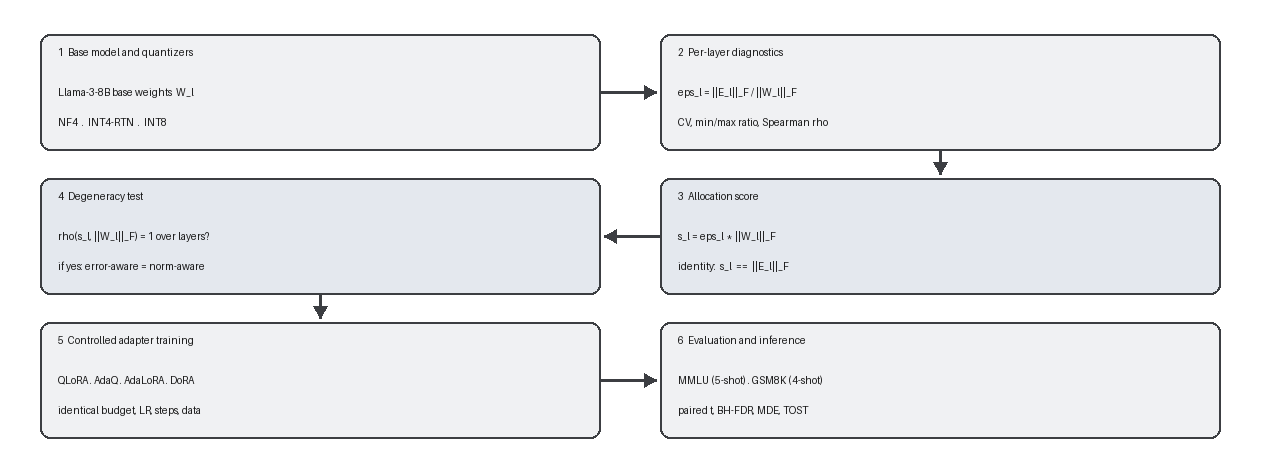
\includegraphics[width=0.78\linewidth]{audit_framework.png}
\caption{Audit protocol. Frozen weights are quantized once per scheme, per-layer diagnostics decide whether the score carries information beyond the weight norm, and the arms are trained identically and compared with seed-matched paired inference. $E_l = W_l-\hat{W}_l$; $\varepsilon_l$: relative error; $s_l = \varepsilon_l\|W_l\|_F$; CV: coefficient of variation.}
\label{fig:framework}
\end{figure}

\begin{algorithm}[t]
\caption{Error-aware rank allocation audit for one quantizer}
\label{alg:audit}
\begin{algorithmic}[1]
\Require frozen weights $\{W_l\}_{l=1}^{L}$; quantizer $Q$; rank budget $R$; seeds $S$; benchmarks $\mathcal{B}$
\Ensure degeneracy diagnostics, per-cell effect estimates, equivalence bounds
\State $\hat{W}_l \gets Q(W_l)$; \ $E_l \gets W_l-\hat{W}_l$; \ $\varepsilon_l \gets \|E_l\|_F/\|W_l\|_F$
\State $\mathrm{CV}_\varepsilon \gets \mathrm{sd}(\varepsilon)/\mathrm{mean}(\varepsilon)$; \ $\rho_s \gets \mathrm{Spearman}(s,\|W\|_F)$
\State $s_l \gets \varepsilon_l\|W_l\|_F$; \ $r_l \gets \mathrm{round}(R\,s_l/\sum_{l'} s_{l'})$; \ $r^{\mathrm{uni}}_l \gets R/L$
\For{$k \in S$}
  \State train all arms with identical hyper-parameters
  \For{$b \in \mathcal{B}$} \State $a_{k,b} \gets \mathrm{evaluate}(\mathrm{arm}_k,b)$ with one shared harness \EndFor
\EndFor
\State paired differences $d_{k,b} = a^{\mathrm{uni}}_{k,b}-a^{\mathrm{err}}_{k,b}$; test $H_0{:}\,\mathbb{E}[d]=0$
\State Benjamini--Hochberg across all $(Q,b)$ cells; report $q$ rather than raw $p$
\State per-cell $\mathrm{MDE}_{80}$ and TOST sample size for SESOI $\delta \in \{0.5,1,2,5\}$
\State \Return diagnostics, $(\hat d,\mathrm{CI}_{95},q,\mathrm{MDE}_{80})$, TOST requirements
\end{algorithmic}
\end{algorithm}

\textbf{Measurements.} We quantize all linear layers of Llama-3-8B~\citep{touvron2024llama3} once per scheme and keep them frozen: NF4 with block-wise absmax scaling (group 64), symmetric INT4 round-to-nearest (group 128), and per-channel INT8. Per scheme we record $\varepsilon_l$, its CV, the max/min ratio, and Spearman correlations among $s_l$, $\varepsilon_l$ and $\|W_l\|_F$. NF4 and INT4-RTN statistics cover the 64 query projections used by the adapter arms; INT8 covers all 226 linear layers, a difference we return to in Section~\ref{sec:obs1}.

\textbf{Arms.} Four arms share one recipe: QLoRA (uniform), the rule of \eqref{eq:score} (denoted AdaQ), AdaLoRA's sensitivity-based allocation, and DoRA's magnitude-direction decomposition. All receive the same total budget of 512 ranks over the same 64 modules (q\_proj and v\_proj), the same training data, learning rate, schedule and optimiser, and the same effective batch size; only the allocation rule differs. Seeds are $\{42,3407,2025\}$ for NF4 and for INT4-RTN MMLU, $\{42,3407,2025,7,100\}$ for INT8, and twelve seeds for INT4-RTN GSM8K (adding 1--7, 100 and 1234); each is an independent training run rather than a re-evaluation of one checkpoint. Cell sizes follow the resolution each claim needs (Section~\ref{sec:power}).

\textbf{Norm-awareness of the realised allocation.} Since $s_l = \varepsilon_l\|W_l\|_F$, layers $i$ and $j$ swap order relative to the norm ranking only if $\|W_i\|_F/\|W_j\|_F \in (\varepsilon_j/\varepsilon_i,\ \varepsilon_i/\varepsilon_j)$, an interval of width $\approx 2\,\mathrm{CV}$. With the measured NF4 CV this is about 3\%: the rankings can differ only among pairs whose norms agree to within a few percent, and such pairs receive nearly identical ranks anyway. We therefore do not add a separate norm-aware arm, which under the measured dispersion would duplicate the error-aware arm (empirical correlate $\rho = 0.998$).

\textbf{Analysis.} Per quantizer--benchmark cell we run a two-sided paired Student $t$ test on seed-matched differences $d_s = a^{\mathrm{uni}}_s - a^{\mathrm{err}}_s$ (negative favouring AdaQ), with Cohen's $d$ for paired data, a $t$-based 95\% interval and the minimum detectable effect at $\alpha = 0.05$, power $0.8$. We test six cells, so we correct the raw $p$ values by Benjamini--Hochberg~\citep{benjamini1995fdr} and $q$ is the statistic; in the cells with three seeds no non-parametric test can reach conventional significance (the smallest attainable two-sided $p$ is 0.25), so none is used as a primary test and no significance stars appear. We judge equivalence by comparing each interval with a smallest effect size of interest (SESOI) in the TOST framework~\citep{lakens2018equivalence}. All decisions are fixed by this protocol: no cell is dropped and no benchmark added after inspection~\citep{simmons2011falsepositive,kerr1998harking}, and effects are reported with uncertainty rather than $p$ alone~\citep{wasserstein2016asa}.

%% =============================================================================
\section{Results}
\label{sec:results}

\subsection{Per-layer error is near-constant at 4 bits}
\label{sec:obs1}

Fig.~\ref{fig:epsilon} gives the error profiles. Under NF4 and INT4-RTN relative error is essentially flat across the 64 query projections (mean $0.094$ and $0.090$, CV 1.48\% and 0.48\%, max/min 1.09 and 1.03). Under INT8, over all 226 linear layers, the mean falls to $0.065$ while dispersion rises sharply (CV 61.1\%, max/min 12.2); because this layer set also includes embeddings and the output head, its dispersion is not directly comparable with the 4-bit rows. The two 4-bit schemes rank layers consistently: their per-layer errors correlate at $\rho = 0.887$ ($p = 1.9\times10^{-22}$, $n = 64$).

\begin{figure}[t]
\centering
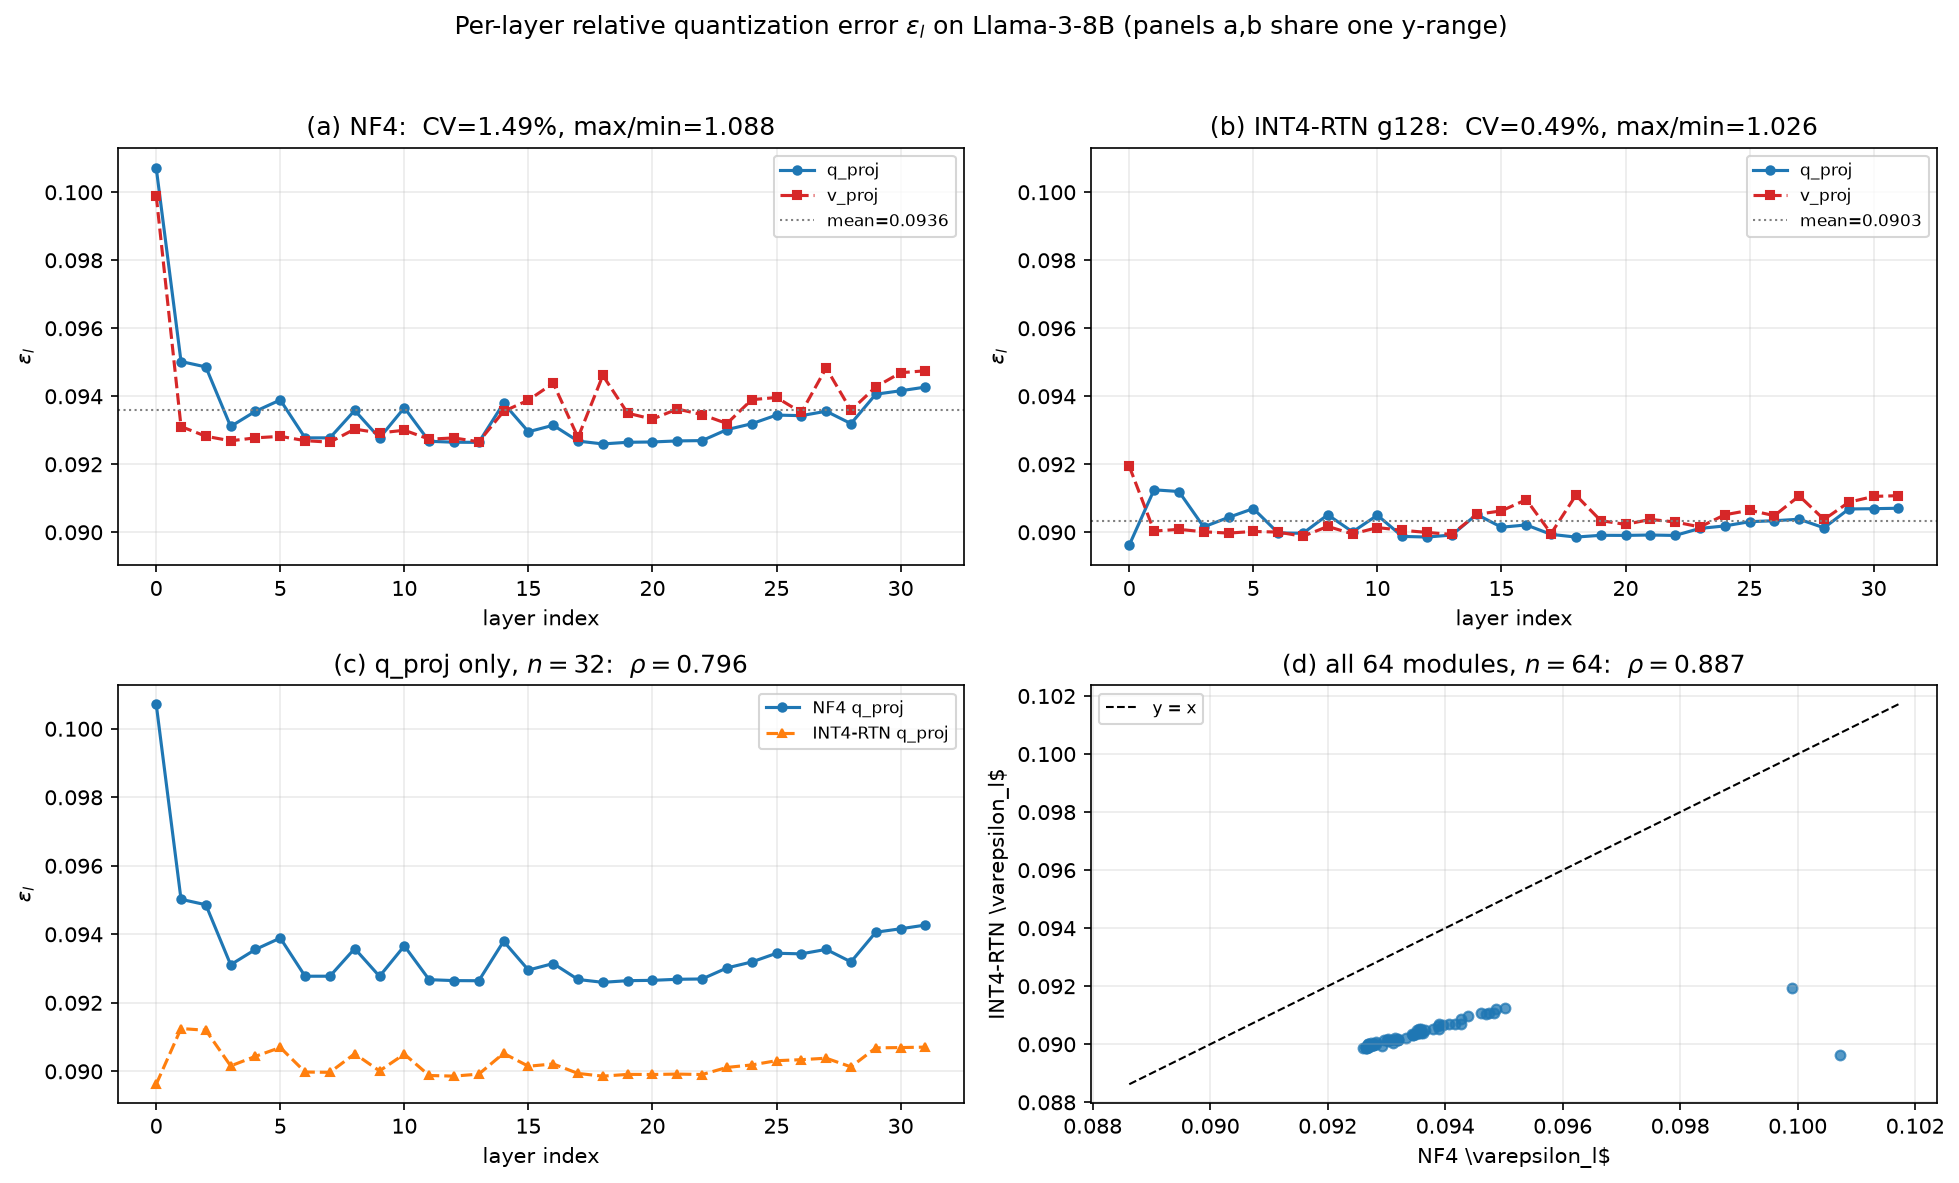
\includegraphics[width=0.62\linewidth]{epsilon_cross_quantizer.png}
\caption{Per-layer relative error $\varepsilon_l$ on Llama-3-8B. (a) NF4, CV = 1.48\%. (b) INT4-RTN, CV = 0.48\%. (c) Overlay on the shared query projections. (d) Cross-quantizer scatter, $\rho = 0.887$ ($n = 64$). Panels (c)--(d) use the 64-layer common subset; the INT8 statistics use all 226 linear layers.}
\label{fig:epsilon}
\end{figure}

The flatness follows from three properties of 4-bit weight quantization: block-wise absmax scaling removes inter-block scale variation, pre-trained weights are close to Gaussian within a block, and the NF4 and INT4 codebooks are designed to be near-optimal for Gaussian inputs. When all three hold, codebook resolution governs relative error, not layer statistics. The mechanism also predicts where the regularity breaks---layers that are not Gaussian, such as embeddings and the output head, which is what the wider INT8 layer set exposes.

\subsection{The score collapses to the error norm}
\label{sec:obs2}

Eq.~\eqref{eq:degeneracy} fixes the score to $\|E_l\|_F$; the measurement shows what this does to the ranking. The Spearman correlation between $s_l$ and $\|W_l\|_F$ is $0.998$ for both 4-bit schemes, while the correlation with $\varepsilon_l$ is $0.144$ (NF4) and $-0.084$ (INT4-RTN); regressing out the norm leaves $R^2_{\Delta\varepsilon} < 0.0005$. Under INT8, where dispersion is much larger, the score still does not separate from the norm because $\varepsilon_l$ is uncorrelated with $\|W_l\|_F$ ($|\rho| < 0.09$). Error-aware allocation is, in this regime, norm-aware allocation.

\subsection{No significant difference from uniform allocation}
\label{sec:main}

Table~\ref{tab:main_results} reports the primary comparison, computed from per-seed records. No cell is significant after false-discovery-rate control ($q \geq 0.20$), and the two smallest raw $p$ values, 0.073 (NF4 MMLU) and 0.075 (INT8 GSM8K), point in opposite directions.

\begin{table}[t]
\centering
\caption{Uniform (QLoRA) versus error-aware (AdaQ) allocation, seed-matched. $\Delta = \mathrm{QLoRA}-\mathrm{AdaQ}$, negative values favouring AdaQ; all quantities in percentage points (pp). $q$: Benjamini--Hochberg adjusted $p$ over six cells; MDE: minimum detectable effect ($\alpha=0.05$, power $0.8$). $n$: seeds, INT4-RTN GSM8K using twelve for a wider sample (Section~\ref{sec:power}).}
\label{tab:main_results}
\footnotesize
\setlength{\tabcolsep}{4.5pt}
\begin{tabular}{llcccccc}
\toprule
\textbf{Quantizer} & \textbf{Benchmark} & \textbf{$n$} & \textbf{$\Delta$ (pp)} & \textbf{95\% CI} & \textbf{$d$} & \textbf{$q$} & \textbf{MDE (pp)} \\
\midrule
NF4      & MMLU  & 3 & $-0.07$ & [$-$0.16, $+$0.02] & $-2.02$ & 0.202 & 0.11 \\
NF4      & GSM8K & 3 & $-0.55$ & [$-$1.52, $+$0.42] & $-1.41$ & 0.202 & 1.21 \\
INT4-RTN & MMLU  & 3 & $-0.12$ & [$-$0.38, $+$0.15] & $-1.10$ & 0.236 & 0.33 \\
INT4-RTN & GSM8K & 12 & $-0.64$ & [$-$1.52, $+$0.23] & $-0.47$ & 0.202 & 1.22 \\
INT8     & MMLU  & 5 & $+0.02$ & [$-$0.34, $+$0.37] & $+0.06$ & 0.907 & 0.48 \\
INT8     & GSM8K & 5 & $+1.46$ & [$-$0.24, $+$3.15] & $+1.07$ & 0.202 & 2.27 \\
\bottomrule
\end{tabular}
\end{table}

Every interval contains zero, and on MMLU the intervals are narrower than 0.75 points for all three quantizers, excluding differences of practical interest. The two nominal near-significant cells have opposite signs, as expected when the underlying effect is near zero and seed noise dominates. Cohen's $d$ is large in several cells (up to 2.02) while the differences are fractions of a point: with few seeds the standardised effect has a small denominator and is uninformative here~\citep{cohen1988}, so we report it only for completeness. GSM8K is far noisier than MMLU in this pipeline: for a fixed arm, per-seed strict-match accuracy ranges over up to 13 points, yet seeds move both arms together, so the paired difference varies by only 0.4--1.4 points.

\subsection{Four-arm comparison under NF4}
\label{sec:full_comparison}

Under NF4 the four arms are indistinguishable: MMLU 0.6533, 0.6540, 0.6538 and 0.6543; GSM8K 0.4711, 0.4766, 0.4774 and 0.4799 for QLoRA, AdaQ, AdaLoRA and DoRA (seed s.d. at most 0.0015 and 0.0055). All lie within 0.10 and 0.88 points, and DoRA's lead costs 30\% more trainable parameters.

\subsection{What the design resolves}
\label{sec:power}

Since the interesting claim is an absence, we state resolution explicitly instead of resting on non-significance. On MMLU the 95\% intervals lie inside $\pm 0.5$ points for all three quantizers (NF4 $[-0.16,+0.02]$, INT4-RTN $[-0.38,+0.15]$, INT8 $[-0.34,+0.37]$), so we conclude equivalence within half a point, a stronger statement than the absence of a significant difference. This margin is read off the observed interval rather than pre-specified, so we treat it as a descriptive equivalence bound rather than a confirmatory TOST rejection. On GSM8K the intervals support equivalence within $\pm 2$ points for both 4-bit schemes and within $\pm 3.2$ points for INT8, so a two-point effect is excluded for the 4-bit quantizers but not for INT8. Given the observed within-cell variability, a pre-planned TOST at $\delta = 1$ point with 80\% power needs at most 3 seeds on MMLU (already met), about 14 on GSM8K for either 4-bit scheme, and five for INT8 at $\delta = 2$ points. Repeating the GSM8K cells under flexible answer extraction leaves the conclusions unchanged (INT4-RTN $\Delta = -0.61$, $q = 0.15$; INT8 $\Delta = +0.85$, $q = 0.39$), so the null result is not an artefact of the stricter scorer.

%% =============================================================================
\section{Discussion}
\label{sec:discussion}

\textbf{Why the rule has no room to act.} An allocation rule helps only if the quantity it ranks by varies enough to change the realised ranks, and if marginal return to rank depends on that quantity. At 4 bits the first condition fails: relative error varies by under 1.5\% across layers, so the induced ranking is the norm ranking up to pairs whose norms agree to within a few percent. This follows from block-wise scaling plus near-Gaussian weights, which is why two independent 4-bit schemes give flat profiles correlating at $\rho = 0.887$; it is not specific to NF4 or to one implementation. INT8 seems to offer an escape, but there the second condition fails: the layers with the largest relative error are not those with the largest norm ($|\rho| < 0.09$), so the error term adds a component uncorrelated with the importance proxy it is meant to modulate. Dispersion in a direction that carries no information about adaptation benefit does not create signal: variance is necessary but not sufficient, it must align with marginal return to rank.

\textbf{Implications.} First, \emph{norm-aware is the appropriate baseline}: because the score equals the error norm and, at 4 bits, tracks the weight norm closely, a comparison against uniform allocation alone cannot separate error-awareness from norm-awareness. Adaptive-rank papers should report the correlation between their statistic and the weight norm, a one-line diagnostic that would have exposed this degeneracy before any training run. Second, \emph{bit-width determines whether the signal exists}: results at 2 bits, where error is large and heterogeneous~\citep{kim2024ralora,lee2025rilq,chee2023quip}, do not transfer automatically to 4--8 bits, so papers proposing per-layer signals should state the bit-width range at which the signal was verified. Third, \emph{reporting the resolution achieved is what makes a null result usable}: our bounds exclude differences beyond 0.5 points on MMLU and 2 points on GSM8K, which is the part a reader can build on.

\textbf{Threats to validity.} All experiments use Llama-3-8B; architectures with different weight statistics may show less flat profiles, and while the mechanism predicts which models are at risk, we have not tested that prediction. Three to twelve seeds resolve MMLU to half a point and GSM8K to between 2 and 3.2 points, so smaller effects remain untested and we do not claim they are absent. For AdaLoRA and DoRA we reproduce the allocation rule inside a shared pipeline rather than the complete published method, so those arms characterise allocation behaviour under matched conditions rather than the published methods at their best. MMLU and GSM8K probe knowledge and multi-step reasoning; generation quality, instruction following~\citep{zhou2023ifeval} and domain adaptation are outside our evidence, and instruction-tuned evaluation was avoided because the base model degrades under chat templates. 

%% =============================================================================
\section{Conclusion}
\label{sec:conclusion}

We audited the hypothesis that per-layer quantization error guides rank allocation in quantized LoRA. It fails for a structural reason rather than for want of tuning: the score equals the Frobenius norm of the error matrix by algebra, and at 4 bits the relative error is so uniform that the score is, to three decimal places of rank correlation, the weight norm. Seed-matched comparisons across NF4, INT4-RTN and INT8 on MMLU and GSM8K show no significant advantage of error-aware over uniform allocation after false-discovery-rate control, with equivalence within $\pm 0.5$ points on MMLU and $\pm 2$ points on GSM8K for both 4-bit schemes. Where the design is less resolving we state the bound we have rather than a claim we cannot support, and give the sample sizes needed to close the gap. The constructive reading is that quantization error is not a useful per-layer signal at these bit-widths, and that adaptive-rank research should either justify its signal against the norm baseline or move to regimes where the signal's variance aligns with adaptation benefit.

\noindent\textbf{CRediT authorship contribution statement.} {\small\textbf{Yibo Zhang:} Conceptualization, Methodology, Software, Formal analysis, Investigation, Writing -- original draft. \textbf{Muhammad Syafiq bin Mohd Pozi:} Supervision. \textbf{Osman B Ghazali:} Supervision.}

\noindent\textbf{Declaration of competing interest.} {\small The authors declare that they have no known competing financial interests or personal relationships that could have appeared to influence the work reported in this paper.}

\noindent\textbf{Funding.} {\small The authors received no specific funding for this work.}

\noindent\textbf{Declaration of generative AI and AI-assisted technologies in the writing process.} {\small During the preparation of this work the authors used a large language model for language editing and for assistance with analysis scripts. All numerical results were checked against the raw per-seed evaluation records by the authors, who take full responsibility for the content of the publication.}

\noindent\textbf{Data availability.} {\small Code, per-seed evaluation records and the scripts that generate every table in this paper are available from the corresponding author on reasonable request; the project repository will be made public at \url{https://github.com/BRAD-cording/AdaQ-LoRA} upon acceptance.}

%% =============================================================================
\appendix
\section{Training and evaluation configuration}
\label{app:config}

Table~\ref{tab:training_config} lists the configuration shared by all arms; only the allocation rule differs.

\begin{table}[!ht]
\centering
\caption{Training and evaluation configuration for all arms.}
\label{tab:training_config}
\footnotesize
\begin{tabular}{lp{9.2cm}}
\toprule
\textbf{Parameter} & \textbf{Value} \\
\midrule
Base model    & Meta-Llama-3-8B (base, no chat template) \\
Quantization  & NF4 bnb 4-bit (group 64) / INT4-RTN g128 (pre-quantised, loaded in bf16) / INT8 per-channel \\
Adapters      & q\_proj and v\_proj, 64 modules, $\alpha=2r$; budget 512 per-layer from \texttt{ranks.json}, uniform arms rank 8 per module \\
Optimisation  & $2\times10^{-4}$ AdamW, cosine schedule, 3\% warmup, 3 epochs (63 packed steps); batch 1 $\times$ accumulation 16 (NF4 arm: 4 $\times$ 4, same effective batch) \\
Data          & OpenHermes-2.5, first 2000 samples, packed to 2048-token sequences~\citep{teknium2023openhermes} \\
Seeds         & 42, 3407, 2025 for NF4 and INT4-RTN MMLU; 42, 3407, 2025, 1--7, 100, 1234 for INT4-RTN GSM8K; plus 7, 100 for INT8 \\
Compute       & 2 $\times$ RTX 4090 D (24 GB), peak 19.8 GB per run; PyTorch 2.11.0, CUDA 13.0, peft 0.21.2, bitsandbytes 0.50.2, lm-evaluation-harness 0.4.13 \\
Benchmarks    & MMLU 5-shot, 14042 items~\citep{hendrycks2021mmlu}; GSM8K 5-shot, 1319 items, strict-match primary~\citep{cobbe2021gsm8k} \\
\bottomrule
\end{tabular}
\end{table}

For AdaQ, ranks are proportional to $s_l = \varepsilon_l\|W_l\|_F$ within each projection type, normalised to the budget; QLoRA splits the budget uniformly. The AdaLoRA arm uses its sensitivity score to allocate ranks but keeps our training objective, since the full formulation (incremental SVD with orthogonality regularisation) is incompatible with a fixed-rank $BA$ parameterisation; it therefore measures the allocation rule, not the complete method. The DoRA arm decomposes each adapted weight into magnitude and direction and allocates the budget uniformly over the direction component. All arms use $\alpha = 2r$, removing the $\alpha/r$ scaling confound. GSM8K uses strict matching as the primary analysis, with the flexible-extraction check in Section~\ref{sec:power}.

%% =============================================================================
\bibliographystyle{elsarticle-num}
\bibliography{references}

\end{document}
